%&latex
%
\documentclass[../template.tex]{subfiles}
\usepackage{graphicx}

\begin{document}

\section{Introduction}
Modeling a natural phenomenon consists of linking its elements to \textit{abstractions} in a \textit{logical system} in order to deduce its properties or behaviour. For example, to compute the distance between two cities, we think of them as \textit{geometrical points} of no dimension, and then use spherical geometry to determine the length of the great-circle connecting them.  

\medskip

A model is said to be \textbf{deterministic} if it predicts a single outcome from a given set of circumstances. On the other hand, a \textbf{stochastic} model predicts a set of possible outcomes weighted by their \textit{plausibility} - or \textit{probabilities}.   

\medskip

In general, there is no thing as a \textbf{best model} for any given phenomenon. What to use in what circumstance is an arbitrary choice, directed by seeking the most \textit{usefulness} for a specific task of interest. A useful model is one that reflect all aspects of the phenomenon under study that are relevant to the question at hand, and that allow us to make calculations and predictions.

\section{Stochastic Processes}
A \textbf{stochastic process}\index{Stochastic process}\marginpar{Stochastic process} is a family of random variables $X_t$, where $t$ is a parameter running over a suitable index set $T$. We could interpret it as a \q{stochastic function}, that maps an independent variable $t \in T$ to a random outcome $X(t) \in S$ - so that its graph \textit{changes} every time we run the experiment.  

\medskip

$T$ may be a \textbf{discrete}  set\marginpar{Index set} - for example $T = \mathbb{N}$ and $X(n)$ being the outcome of the $n$-th dice toss - or a \textbf{continuos} set - for example $T=[0,\infty)$ and $X(t) = $ temperature at time $t$ at a weather station. \medskip

$T$ does not need to be a \textit{time} or \textit{iteration number}. For example, we could model an image as a stochastic process, with $\bm{t} = (t_1,t_2)$ being the coordinates of a pixel (so, more like a \textit{spatial} index). However, in this course we will limit ourselves to the $d=1$ case.

\medskip

The possible\marginpar{State space} values of $X(t)$ lie in a space $S$ denoted as the \textbf{state space}. For example, for a temperature we have $S=[0,\infty)$, while for a dice toss $S=\{1,2,3,4,5,6\}$.

\medskip

A stochastic process with \textbf{discrete index}\marginpar{Chain} and \textbf{discrete state space} is called a \textbf{chain}\index{Chain}.

\medskip

To describe a stochastic process, we may start by specifying the \textit{statistics} of each random variable $X_t$ - for example their distribution. If all $X_t$ distribute the same, the process is said to be \textbf{stationary}. 

In the general case, however, $X_t$ and $X_{t'}$ at different\marginpar{Joint distribution} times $t\neq t'$ may be correlated, meaning that the distribution of the latter \textit{depends} on the outcome of the former. So, a \textbf{full description} of a stochastic process necessarily involves knowing the \textbf{joint distribution} of any set $\{X_t \colon t \in \bar{T}\}$ for any subset $\bar{T} \subseteq T$. 

This is clearly a huge amount of information, especially if $T$ is continuous. Fortunately, in many cases, stochastic processes possess some \textit{special properties} that allow to describe them fully with only a few parameters. 

\section{Quick Review of Probability Theory}
Recall the main concepts of probability theory:\marginpar{Main definitions}
\begin{itemize}
    \item \textbf{Sample space}: set of all possible outcomes of an experiment, usually denoted with $\Omega$
    \item \textbf{Event}: any subset of $E \subseteq \Omega$
    \item \textbf{Probability}: a \textit{measure} of events, i.e. a way to associate any event $E$ to a real positive number $\mathbb{P}[E] \in [0,1]$. We have $\mathbb{P}[\Omega] = 1$ and $\mathbb{P}[\varnothing] = 0$.   
\end{itemize}
If $A$ and $B$ are events, their union $A \cup B$ is the event representing the realization of either $A$, $B$ or both. To measure its size (probability) we need to pay attention not to count two times the intersection of $A$ and $B$, and so:
\begin{align*}
    \mathbb{P}[A \cup B] = \mathbb{P}[A] + \mathbb{P}[B] - \mathbb{P}[A \cap B]
\end{align*}

Consider a disjoint partition $\{A_i\}$ of the sample space $\Omega$:
\begin{align*}
    \bigcup_{i} A_i = \Omega; \qquad \mathbb{P}[\Omega] = 1; \qquad A_i \cap A_j = \varnothing\quad \forall i \neq j
\end{align*}
We can rewrite the probability of any event $B$ as the sum of its \textit{intersections} with the partition elements $A_i$, leading to the \textbf{law of total probability}\index{Law!Total probability}\marginpar{Law of total probability}:  
\begin{align*}
    \mathbb{P}[B] = \sum_{i} \mathbb{P}[B \cap A_i]
\end{align*}

Two events are said to be \textbf{independent}\index{Independence}\marginpar{Independent events} if and only if:
\begin{align*}
    \mathbb{P}[A \cap B] = \mathbb{P}[A] \mathbb{P}[B]
\end{align*}
Generalizing, $n$ events are independent if and only if:
\begin{align*}
    \mathbb{P}\left[\bigcup_i^n A_i\right] = \prod_{i}^n \mathbb{P}[A_i]
\end{align*}

\subsection{Random variables}
A \textbf{random variable} is a \q{variable that takes on its values by chance}. It acts as a \q{placeholder} for the outcome of an experiment that may result in a \textit{range} of possible values. For example, we may denote with $X$ the act of \textit{tossing a dice}. After doing the experiment, we obtain, for example, the outcome $4$, and we then say that $X$ \q{assumes} the value of $4$ in this \q{realization} of the experiment.

\medskip

By convention, we denote random variables with capital letters ($X$, $Y$, $Z$), and real numbers with lowercase letters ($x$, $y$, $z$). As an event is just a set of outcomes, we can specify it as a subset of the values that a random variable $X$ may assume. For example $\{X \leq x\}$ is the \textbf{event} that the random variable $X$ assumes a value that is less than or equal to the real number $x$. The \textit{measure} of that set is its probability, denoted with $\mathbb{P}[\{X \leq x\}]$. In this case it is a function of the real number $x$.

\medskip

We define the (cumulative) \textbf{distribution function}\marginpar{Cumulative distribution function (CDF)}\index{Function!Cumulative distribution} of the random variable $X$ as the quantity:
\begin{align*}
    F_X(x) = \mathbb{P}[\{X \leq x\}] \qquad F_X\colon \mathbb{R} \to [0,1]
\end{align*} 
Clearly, $F(-\infty) = 0$, $F(\infty) = 1$ and it is \textit{non-decreasing}: if we rise the value of $x$ we are either including new possible outcomes in the event, or leaving it the same, and so its size (probability) cannot decrease. It can also be shown that $F_X(x)$ is \textit{right}-continuous, meaning that:
\begin{align*}
    \lim_{x \to c^+} F_X(x) = F_X(c) \qquad \forall c \in \mathbb{R}
\end{align*} 
Suppose that $X$ is a \textit{discrete random variable}, meaning that it \q{assumes} values in a discrete set $X \in \{x_n\}_{n \in T}$. Then $F_X(x)$ is a \q{step function}, that is constant in the intervals $[x_{i-1}, x_i)$ and makes \textit{jumps} of size $\mathbb{P}[X=x_i]$ at $x=x_i$, as can be seen in fig. \ref{fig:cdf-discrete}.  

\begin{figure}[htp]
    \begin{subfigure}[t]{0.45\textwidth}
      \centering
      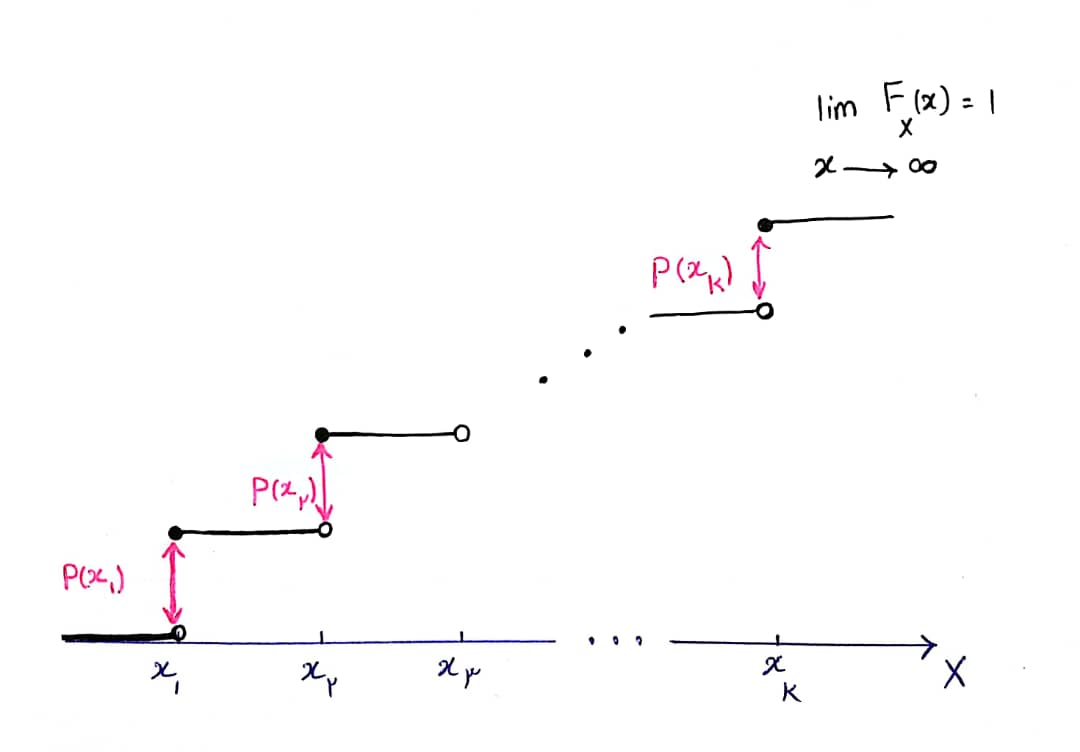
\includegraphics[width=\textwidth]{image001.png}
      \caption{CDF for a discrete random variable\label{fig:cdf-discrete}}
      \label{fig:f1}
    \end{subfigure}
    \hfill
    \begin{subfigure}[t]{0.45\textwidth}
      \centering
      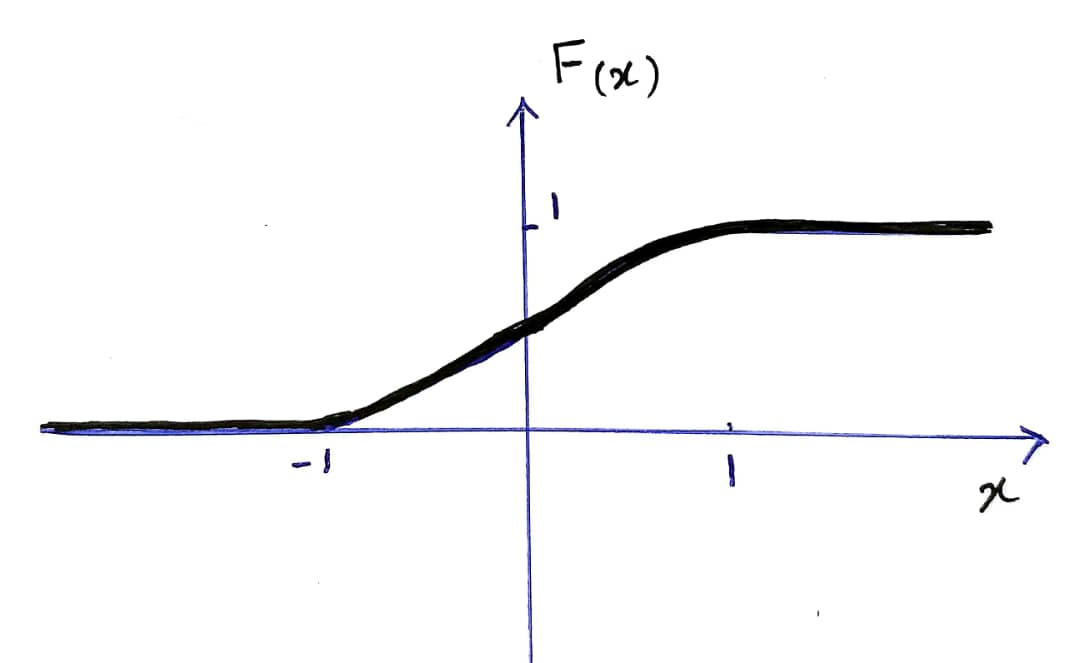
\includegraphics[width=\textwidth]{image002.png}
      \caption{CDF for a continuous random variable\label{fig:cdf-continuous}}
      \label{fig:f2}
    \end{subfigure}
    \caption{Examples of Cumulative Probability Distributions (CDF)\label{fig:cdfs}}
  \end{figure}

If $\mathbb{P}[X=x] = 0$ $\forall x$, then $F_X(x)$ does not make any discontinuous jump, and its graph is continuous (fig. \ref{fig:cdf-continuous}).

\medskip

If $F_X(x)$ is differentiable,\marginpar{PDF} we call its derivative the \textbf{probability density function} (pdf)\index{Function!Probability density}:
\begin{align*}
    f_X(x) \equiv \dv{F_X(x)}{x}
\end{align*} 
Then, from the fundamental theorem of calculus, we have:
\begin{align*}
    F_X(x) = \int_{-\infty}^x f(\xi) \dd{\xi}; \qquad F(b) - F(a) = \mathbb{P}[a < X \leq b] = \int_a^b f(\xi) \dd{\xi}
\end{align*}

\subsection{Moments and Expected Values}
Moments are a way to summarize the \textit{shape} of a distribution with numbers.

\medskip

For a discrete random variable $X$, the $m$-th moment is defined by:\marginpar{Moments}
\begin{align*}
    \mathbb{E}[X^m] = \sum_{i} x_i^m \mathbb{P}[X= x_i]
\end{align*}
where the sum is over all possible values that $X$ can assume. In the continuous case, we substitute the sum with an integral:
\begin{align*}
    \mathbb{E}[X^m] = \int_{-\infty}^{+\infty} x^m f(x) \dd{x}
\end{align*}
The first moment $\mathbb{E}[x]$ is also called the \textbf{mean}\index{Mean}\marginpar{Mean}. 

\medskip

We define the $m$-th \textbf{central moment}\index{Moment!Central}\marginpar{Central moment} as the $m$-th moment of the random variable $X$ obtained \textit{after subtracting its mean}:
\begin{align*}
    \mathbb{E}[(X-\mathbb{E}[X])^m]
\end{align*}  
The second central moment is also called the \textbf{variance}\index{Variance}\marginpar{Variance} of $X$:
\begin{align*}
    \operatorname{Var}[X] = \mathbb{E}[(X-\mathbb{E}[X])^2] 
\end{align*} 

The \textbf{expected value}\marginpar{Expected value} of a function $g(x)$ is defined as:
\begin{align}\label{eqn:measure-discrete}
    \mathbb{E}[g(x)] = \sum_{i} \mathbb{P}[X=x_i] g(x_i)
\end{align} 
in the \textbf{discrete} case, and as:
\begin{align}\label{eqn:measure-continuous}
    \mathbb{E}[g(x)] = \int_{\mathbb{R}} g(x) f(x) \dd{x}
\end{align}
in the \textbf{continuous} case.

\medskip

We can \textit{unify} both definitions by writing:\marginpar{Unique expression}
\begin{align}
    \mathbb{E}[g(x)]  = \int_{\mathbb{R}} g(x) \dd{F(x)}\label{eqn:measure-exp}
\end{align}
The measure $\dd{F(x)}$ has a rigorous mathematical meaning (as a Lebesgue-Stieltjes integral) - but we will simply interpret (\ref{eqn:measure-exp}) as equivalent to either (\ref{eqn:measure-discrete}) or (\ref{eqn:measure-continuous}) depending on the \textit{nature} of the random variable $X$ at hand. 

\subsubsection{Many variables}
We can generalize everything to \textbf{multiple dimensions}.\marginpar{Many variables} For example, given a pair $(X,Y)$ of random variables, their \textbf{joint} (cumulative) distribution function is defined as:
\begin{align*}
    F_{XY}(x,y) = F(x,y) = \mathbb{P}[X \leq x \text{ and } Y \leq y]
\end{align*} 

Two random variables $X$ and $Y$ are said to be \textbf{independent} if their joint distribution function \textit{factorizes} everywhere:
\begin{align} \label{eqn:independence}
    X, Y \text{ are independent} \Leftrightarrow F(x,y) = F_X(x) F_Y(Y) \quad \forall x,y
\end{align}
The same happens with their \textit{pdf}s.

\medskip

A related concept is that of \textbf{correlation}.\index{Correlation}\marginpar{Correlation} Specifically, $X$ and $Y$ are said to be \textbf{uncorrelated} if the expectation of their product (after removing the mean) is null:
\begin{align} \label{eqn:correlation}
    \mathbb{E}[(X-\mu_X)(Y-\mu_Y)] = 0 \qquad \mu_X=\mathbb{E}[X], \> \mu_Y = \mathbb{E}[Y]
\end{align}  
We note that \textbf{independence} implies \textbf{uncorrelation},\marginpar{Independence $\Rightarrow$ Uncorrelation} but the converse is not true.  In fact, by linearity of the expected value we can expand (\ref{eqn:correlation}) to:
\begin{align*}
    \mathbb{E}[(X-\mu_X)(Y-\mu_Y)] &= \mathbb{E}[XY] - \mu_X \underbrace{\mathbb{E}[Y] }_{\mu_Y}- \mu_Y\underbrace{\mathbb{E}[X]}_{\mu_X}+ \mu_X \mu_Y
\shortintertext{and then use the independence property (\ref{eqn:independence}) to factorize the expectation $\mathbb{E}[XY] = \mathbb{E}[X] \mathbb{E}[Y] = \mu_X \mu_Y$, so that:}
    &= \bcancel{\mu_X \mu_Y }-\bcancel{ \mu_X \mu_Y} -\cancel{ \mu_Y \mu_X }+ \cancel{\mu_X \mu_Y} = 0
\end{align*}

\subsubsection{Sum of variables}
Consider the sum $Z=X+Y$ of two random variables $X$ and $Y$. Then:
\begin{align*}
   F_Z(z) = \mathbb{P}[Z \leq z] &= \mathbb{P}[X+Y \leq z] \underset{(a)}{=}  \mathbb{E}_Y[P[X+Y \leq z|Y]] =\\
    &= \mathbb{E}_Y [\mathbb{P}[X \leq z- Y| Y]] \underset{(b)}{=}  \mathbb{E}_Y[F_X(z-Y)] = \\
    &\underset{(\ref{eqn:measure-exp})}{=}  \int_{\mathbb{R}} F_X(z-\xi) \dd{F_Y(\xi)}
\end{align*}
where in (a) we are taking the \textit{average} over all \textit{conditional probabilities} (which is just an application of the law of total probability), and the in (b) we recognize the distribution function of $X$, evaluated at $z-Y$.

\medskip

Note that nothing changes if we exchange the roles of $X$ and $Y$, and so:
\begin{align*}
    F_Z(z) = \int_{\mathbb{R}} F_Y(z-\eta) \dd{F_X}(\eta)
\end{align*}
This final operation is a \textit{convolution}. We can see it explicitly if we suppose that $X$ and $Y$ have \textit{pdf}s, so that:
\begin{align*}
    F_Z(z) = \int_{\mathbb{R}} F_X(z- \xi)
\end{align*}

Then we can take the derivative:
\begin{align*}
    f_Z(z) &= \dv{F_z(z)}{z} = \int_{\mathbb{R}} \dv{z} F_X(z-\xi) \dd{F_Y(\xi)} = \int_{\mathbb{R}} f_X(z- \xi) \dd{F_Y(\xi)} =\\
    &\underset{(\ref{eqn:measure-continuous})}{=} \int_{\mathbb{R}} f_X(z- \xi) f_Y(\xi)
\end{align*}  

In general:
\begin{align*}
    \mathbb{E}[X+Y] &= \mathbb{E}[X] + \mathbb{E}[Y] \qquad \text{always}\\
    \operatorname{Var}[X+Y] &= \operatorname{Var}[X] + \operatorname{Var}[Y] \qquad \text{if $X,Y$ are uncorrelated}   
\end{align*}
(Prove it as exercise)

\subsubsection{Conditional probabilities}
Previously, we used the concept of a \textit{conditional probability}, that we now define precisely.

For any events $A$ and $B$, the \textit{conditional probability} of $A$ given $B$ is written $\mathbb{P}[A|B]$ and defined by:
\begin{align*}
    \mathbb{P}[A|B] = \frac{\mathbb{P}[A \cap B]}{\mathbb{P}[B]} \qquad \text{if } \mathbb{P}[B] > 0
\end{align*} 
Then, substituting this definition in the \textbf{law of total probability} we arrive to:
\begin{align*}
    \mathbb{P}[A] = \sum_{i} \mathbb{P}[A|B_i] \mathbb{P}[B_i]
\end{align*} 
where $B_i$ are a disjoint partition of the sample space $\Omega$.
\end{document}
